\chapter{Simulation of on-~and off-shell \ttbartitle production with \texorpdfstring{\bbfourl}{bb4l}}
\label{ch:bb4l}

\section{Introduction}

The accurate modeling of top quark production processes at the LHC is of crucial importance for precision measurement of top quark properties. In particular, the fact the top quark is an unstable resonance with a short lifetime presents challenges for correctly modeling its mass lineshape as used for top mass and width measurements~\cite{Tarrach:1980up,Smith:1996xz,Hoang:2020iah}. Typically, the modeling is done with full NLO MC simulations matched to a parton shower (NLO+PS), and multiple such generators are available with different features and degrees of accuracy.

In this chapter, the predictions of some of these generators from the \powheg framework~\cite{Powheg:2004,Powheg:2007} are compared to each other, as well as to unfolded data measured in \citere{ATLAS:2018ivx}, for different variables relevant to top mass and/or width measurements. A particular focus is the generator \bbfourl \cite{Jezo:2016ujg}, which specifically improves the treatment of the unstable top resonance and of the interference between \ttbar and tW, and is described in detail in \cref{sec:bb4l:bb4l}. In this work, \bbfourl is implemented and validated for the first time in the CMS simulation setup. The comparison is done at the generator level, i.e. including parton showering and hadronization but not detector simulation and experimental reconstruction.

The results of this work have been published in a CMS public note as \citere{CMS:NOTE-2023-015}. Since the publication of this note, a new version of \bbfourl has been made available~\cite{Jezo:2023rht}, leading to small differences as discussed below. In this thesis, updated results including both versions will be shown.

\section{The Monte Carlo generator \texorpdfstring{\bbfourl}{bb4l}}
\label{sec:bb4l:bb4l}

\bbfourl ~\cite{Jezo:2016ujg,Jezo:2023rht} is a full NLO+PS MC generator for the process $pp \to b \bar{b} \ell^+ \ell^- \nu_\ell \bar{\nu}_\ell$, including all off-shell contributions. This includes the dilepton decay channel of both \ttbar and tW production, as well as non-resonant contributions involving Z or Higgs bosons, as shown in \cref{fig:bb4l:feynman}. Since these processes all lead to the same final state at NLO in QCD, they interfere which each other and can not be easily seperated. \bbfourl includes this interference by construction since it computes the full amplitude including all diagrams at once.

\begin{figure}[t]
    \centering
    \begin{tikzpicture}[baseline=(current bounding box.center)]
      \begin{feynman}
        \vertex (i1) {\(g\)};
        \vertex [below=2.0 cm of i1] (i2) {\(g\)};
        \vertex [right=1.5 cm of i1] (a);
        \vertex [right=1.5 cm of i2] (b);
        \vertex [right=1.0 cm of a] (c);
        \vertex [right=1.0 cm of b] (d);
        \vertex [above right=0.15 cm and 0.75 cm of c] (fb1) {\(b\)};
        \vertex [below right=0.15 cm and 0.75 cm of c] (fW1) {\(W^+\)};
        \vertex [above right=0.15 cm and 0.75 cm of d] (fW2) {\(W^-\)};
        \vertex [below right=0.15 cm and 0.75 cm of d] (fb2) {\(\bar{b}\)};
        \diagram* {
          (i1) -- [gluon] (a),
          (i2) -- [gluon] (b),
          (c) -- [anti fermion, edge label'=\(t\)] (a) -- [anti fermion, edge label'=\(t\)] (b) -- [anti fermion, edge label'=\(\bar{t}\)] (d),
          (c) -- [fermion] (fb1),
          (c) -- [boson] (fW1),
          (d) -- [anti fermion] (fb2),
          (d) -- [boson] (fW2),
        };
      \end{feynman}
    \end{tikzpicture}
    \hfill
    \begin{tikzpicture}[baseline=(current bounding box.center)]
      \begin{feynman}
        \vertex (i1) {\(g\)};
        \vertex [right=1.5 cm of i1] (a);
        \vertex [below=2.0 cm of i1] (i2) {\(g\)};
        \vertex [below=1.25 cm of a] (b);
        \vertex [right=1.0 cm of a] (c);
        \vertex [right=1.0 cm of i2] (d);
        \vertex [above right=0.15 cm and 0.75 cm of c] (fb1) {\(b\)};
        \vertex [below right=0.15 cm and 0.75 cm of c] (fW1) {\(W^+\)};
        \vertex [right=1.75 cm of b] (fW2) {\(W^-\)};
        \vertex [right=2.25 cm of d] (fb2) {\(\bar{b}\)};
        \diagram* {
          (i1) -- [gluon] (a),
          (i2) -- [gluon] (d),
          (c) -- [anti fermion, edge label'=\(t\)] (a) -- [anti fermion, edge label'=\(t\)] (b) -- [anti fermion, edge label'=\(b\)] (d),
          (c) -- [fermion] (fb1),
          (c) -- [boson] (fW1),
          (d) -- [anti fermion] (fb2),
          (b) -- [boson] (fW2),
        };
      \end{feynman}
    \end{tikzpicture}
    \hfill
    \begin{tikzpicture}[baseline=(current bounding box.center)]
      \begin{feynman}
        \vertex (i1) {\(g\)};
        \vertex [below=2.0 cm of i1] (i2) {\(g\)};
        \vertex [right=1.5 cm of i1] (a);
        \vertex [right=1.5 cm of i2] (b);
        \vertex [below=1.0 cm of a] (c);
        \vertex [right=1.0 cm of c] (d);
        \vertex [right=2.0 cm of a] (fb1) {\(b\)};
        \vertex [above right=0.15 cm and 0.75 cm of d] (fW2) {\(W^+\)};
        \vertex [below right=0.15 cm and 0.75 cm of d] (fW1) {\(W^-\)};
        \vertex [right=2.0 cm of b] (fb2) {\(\bar{b}\)};
        \diagram* {
          (i1) -- [gluon] (a),
          (i2) -- [gluon] (b),
          (fb1) -- [anti fermion] (a) -- [anti fermion, edge label'=\(b\)] (c) -- [anti fermion, edge label'=\(b\)] (b) -- [anti fermion] (fb2),
          (c) -- [boson, edge label'=\(Z\mathrm{,}\gamma\)] (d),
          (d) -- [boson] (fW1),
          (d) -- [boson] (fW2),
        };
      \end{feynman}
    \end{tikzpicture}
    \caption{\textbf{Feynman diagrams for \bbfourl.} Examples of Feynman diagrams for the $pp \to b \bar{b} W^+ W^-$ process as described by \bbfourl, including double-resonant (left), single-resonant (center) and non-resonant contributions (right). The decay of the W bosons into leptons is not shown for brevity.}
    \label{fig:bb4l:feynman}
\end{figure}

In addition, by considering the full amplitude instead of splitting it into production and decay parts, \bbfourl fully treats the top quark as an unstable resonance without approximations. It is implemented in the ``resonance-aware'' version of \powheg, called \powhegvres~\cite{Jezo:2015aia}, which includes hard QCD radiation also for unstable resonances - such as top quarks - in addition to the initial state radiation always provided by \powheg. As a result, an event generated by \bbfourl can have up to three hard emissions at matrix element level. The correct description of these FSR emissions is relevant e.g. for observables related to the mass of the top quark, and can be challenging for parton showers, leading to large uncertainties.

This work investigates two different versions of \bbfourl. The first version is the one originally published in \citere{Jezo:2016ujg} and publically available on the \powheg website~\cite{Powheg:website}. In the following, it will be referred to as \bbfourl v1.

The second version of \bbfourl was recently published in \citere{Jezo:2023rht}. Its most prominent feature compared to the previous version is the addition of the lepton+jets decay channel of \ttbar, i.e. the $b \bar{b} \ell \nu_{\ell} q \bar{q}'$ final state. In addition, it includes several improvements to the dilepton final state, such as avoidance of spurious finite width effects and improved resonance history projectors (see \citere{Jezo:2023rht} for details). At the time of writing this thesis, the new code is not publically available. A preview version was made available to the CMS collaboration by the authors, and the dilepton final state of this version - referred to as \bbfourl v2 - is shown in this work. The lepton+jets final state, on the other hand, was not ready for validation in the preview version, and so could not be included.

\section{Other \ttbartitle Monte Carlo generators}
\label{sec:bb4l:others}

The distributions predicted by \bbfourl are compared to three other MC generators for the \tttW final state, which are briefly presented in this section. All of these are implemented in \powhegvtwo, and as such do not contain explicit treatment of radiation in unstable resonances.

\subsection{\texorpdfstring{\hvq}{hvq}}

\hvq~\cite{Frixione:2007nw}, standing for \textit{heavy quark}, is the standard code used, at the time of writing, by both the ATLAS and CMS collaborations for producing \ttbar MC events. It applies the narrow-width approximation (NWA) to generate stable \ttbar pairs at NLO in QCD, with up to one additional ISR emission. The top quarks are then randomly smeared according to the top quark width, giving an approximate treatment of finite-width effects. Following this, the top quarks are decayed - in this case, in the dilepton channel for all lepton flavors - using internal \powheg routines~\cite{Frixione:2007zp}. These routines work at tree level with NLO matrix element corrections and preserve spin correlations. Further ISR emissions as well as all FSR emissions are handled by the matching to the parton shower.

\subsection{\texorpdfstring{\ST}{ST\_wtch}}

Since \hvq generates only the double-resonant \ttbar amplitude, a second generator has to be used alongside it for the single-resonant tW and \tttW interference contributions. Here, \ST~\cite{Re:2010bp} is used for this purpose. It works very similar to \hvq, also generating a stable tW pair in the NWA, smearing with the top width and decaying the particles using the same routines.

However, in order to at least approximately recover the full $b \bar{b} W^+ W^-$ amplitude, it is necessary to select a scheme for the treatment of the \tttW interference to prevent double-counting. Since the separation between \ttbar and tW is not well defined at NLO, such schemes will to some degree always be ad-hoc and ambiguous. Two such schemes are implemented for \ST, and both are compared in this work: in the first, called diagram removal (DR), all terms involving the square of double-resonant diagrams are simply removed from the squared amplitude. This is the most intuitive choice, but has the disadvantage of not being gauge invariant~\cite{Frixione:2008yi}. The second method, diagram subtraction (DS), keeps double-resonant diagrams in the squared amplitude, and subtracts a gauge invariant counter-term to remove the double counting~\cite{Tait:1999cf,Frixione:2008yi,Re:2010bp}. For both schemes, the prediction of \ST is added to the one of \hvq (together called \tttWsum) to produce distributions that can be compared to \bbfourl.

\subsection{\texorpdfstring{\ttb}{ttb\_NLO\_dec}}

The generator \ttb~\cite{Campbell:2014kua}, similar to \hvq, works in the NWA and thus generates stable \ttbar pairs with ad-hoc smearing. However, unlike \hvq, it is fully NLO-accurate not only in the production, but also in the decay of the top quarks. This means that, like \bbfourl, it generates up to one hard FSR emission per decaying top quark, leading to up to three hard emissions in the final state. 

It also provides an LO-accurate treatment of the \tttW interference by reweighting the generated \ttbar events to the full off-shell LO amplitude. Thus, like \bbfourl, it can be used on its own and does not need to be added together with e.g. \ST, but is expected to work at a lower accuracy since it includes more approximations.

\section{Technical setup}

For all generators, LHE events were generated and then showered and hadronized with the multi-purpose generator \pythia. Wherever possible, the same settings were used for the different generators, an overview of which can be found in \cref{tab:bb4l:settings}. They are mostly identical to the default settings used by CMS for MC generation, as discussed in \citere{CMS:GEN-17-001}.

\begin{table}
\centering
\begin{tabular}{c c}
    Parameter & Value \\
    \hline
    \hline
    \multicolumn{2}{c}{\powheg settings} \\
    Top quark mass & \SI{172.5}{\GeV} \\
    Top quark width & \SI{1.33}{\GeV} \\
    \hdamp & $1.38 \, m_t$~\cite{CMS:TOP-16-021} \\
    PDF set & NNPDF 3.1~\cite{NNPDF:2017mvq}\\
    \hline
    \multicolumn{2}{c}{\pythia settings} \\
    \pythia version & 8.307 \\
    \pythia tune & CP5~\cite{CMS:GEN-17-001}\\
    \hline
    \multicolumn{2}{c}{\texttt{PowhegHooks} settings~\cite{Pythia:2022}} \\
    \texttt{POWHEG:veto} & \texttt{on} \\
    \texttt{POWHEG:pThard} & 0 \\
    \texttt{POWHEG:pTdef} & 1
\end{tabular}
\caption{\textbf{Generator settings.} An overview of the settings for \powheg and \pythia, as well as the matching between them, for all considered generators.}
\label{tab:bb4l:settings}
\end{table}

\subsection{Parton shower matching}
\label{sec:bb4l:matching_theory}

Special care has to be taken regarding the matching of the \powheg ME generators to the parton shower as provided by \pythia.  %In particular, since \powheg already generates events with one or more hard or soft emissions, depending on the process, these configurations must be removed in some form from the \pythia shower to prevent double-counting~\cite{Corke:2010zj}.
For \hvq and \ST, this is accomplished here using a shower veto as described in \cref{sec:mc:showering}, and technically implemented using the \texttt{PowhegHooks} module of \pythia. By default, this module can only handle one ISR emission at matrix element level, and thus needs to be extended for \bbfourl and \ttb, which also contain FSR emissions in the top decay. This was implemented by the \bbfourl authors in the \texttt{PowhegHooksBB4L} module as described in detail in \citere{FerrarioRavasio:2018whr}. A updated form of this module compatible with \bbfourl v2 is used here. Similarly to the ISR case, it is possible to directly start the shower at the energy scale of the \powheg emission, or alternatively employ a veto for emissions above this scale. The latter is used as the default option, and compared to the former in \cref{sec:bb4l:matching}.

%In the naive approach, this is achieved by starting the parton shower in \pythia only at the hardness scale of the emission generated by \powheg (sometimes called ``wimpy shower''). This way, only additional softer emissions are generated by the shower, and double-counting is avoided. However, this works only as long as the hardness scale definitions in \powheg and \pythia are the same. In practice, they are equal approximately but not exactly, leading to possible inaccuracies.

%A more thorough approach can be achieved by always starting the parton shower at the high kinematic limit (``power shower''), calculating the hardness according to the \powheg definition for each generated emission, and vetoing emissions with hardness larger than the emission generated by \powheg. For ISR emissions this method is implemented in \pythia  as part of the \texttt{PowhegHooks} module, and used for all generators considered here.

%For \hvq and \ST, which generate only ISR emissions at ME level, this treatment are sufficient. However, for \bbfourl and \ttb, the veto procedure has to be extended to the FSR emissions generated by \powheg in the top decay. This was implemented by the \bbfourl authors in the \texttt{PowhegHooksBB4L} module, a modified form of which is used here, and described in detail in \citere{FerrarioRavasio:2018whr}. Similarly to the ISR case, it is possible to directly start the shower at the hardness scale of the \powheg emission, or employ a veto for emissions above this scale. The latter is used as the default options, and compared to the former in \cref{sec:bb4l:matching}.

\subsection{Same-flavor leptons}
\label{sec:bb4l:sameflavor}

By default, both versions of \bbfourl generate only dilepton final states with opposite-flavor leptons (electrons, muons or $\tau$ leptons). This is because, in principle, there are additional diagrams contributing to the $b \bar{b} \ell^+ \ell^- \nu_\ell \bar{\nu}_\ell$ amplitude for same-flavor leptons, such as $b \bar{b} ZZ$ with $ZZ \rightarrow \ell^+ \ell^- \nu_\ell \bar{\nu}_\ell$, that are not included in \bbfourl.

In practice, the effect of these diagrams will be small, especially in experimental analyses where a cut is applied to reject resonant same-flavor lepton pairs close to the Z boson mass (compare \cref{sec:ttxs:channels}). To make sure that \bbfourl can be used in CMS for experimental analyses involving all lepton flavors, a relabeling procedure already included in \bbfourl is extended to also produce same-flavor lepton final states, neglecting the aforementioned diagrams. This procedure is used for all \bbfourl distributions shown in this chapter.

\section{Results}

\subsection{Comparison between generators}

In this section, the two \bbfourl versions are compared against each other, as well as to the alternative generators introduced in \cref{sec:bb4l:others}, for different observables. All of these comparisons are done after parton showering and hadronization, but without any detector simulation.

The package \rivet~\cite{Rivet:2019rhm} was used to analyze the events. For some observables, publically available analysis packages were employed, which is stated in the captions of the figures where applicable. Furthermore, some observables include distributions at the jet level, which are obtained by running an anti-$k_\mathrm{T}$ algorithm with distance parameter $\Delta R = 0.4$ (AK4)~\cite{Cacciari:2008gp}.

\paragraph{Lepton observables} To begin the comparison, events with at least two leptons of opposite sign satisfying $\pt > \SI{20}{\GeV}$ and $\abseta < 2.4$ are selected. Photons surrounding the leptons in a small cone of $\Delta R < 0.1$, originating from photon radiation, are clustered together with the leptons (``dressed leptons''). The \pt distributions of the leading and subleading of these two leptons are shown in \cref{fig:bb4l:leppt}. They show good agreement between the generators within the scale uncertainties, with \tttWsum predicting a slightly harder lepton spectrum then the others.

\begin{figure}[tp]
    \centering
    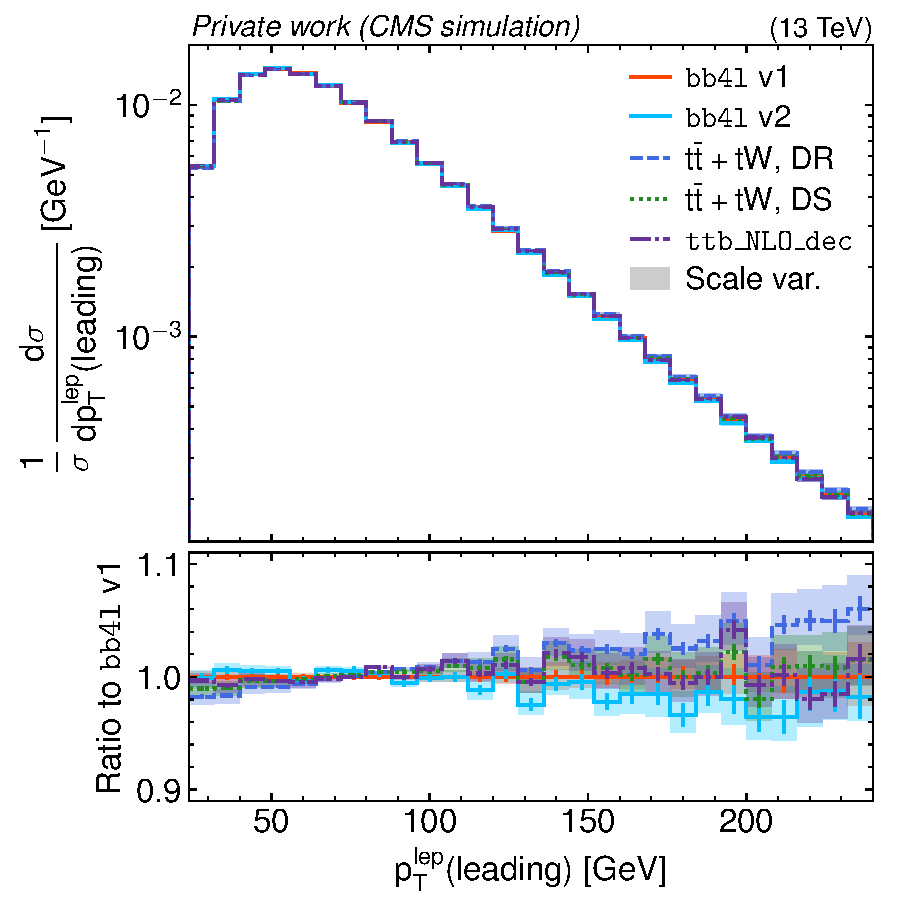
\includegraphics[width=0.49 \textwidth]{figures/bb4l/generators/MC_TTBAR_DILEP_SPINDENSITY_lep_pt_1.pdf}
    \hfill
    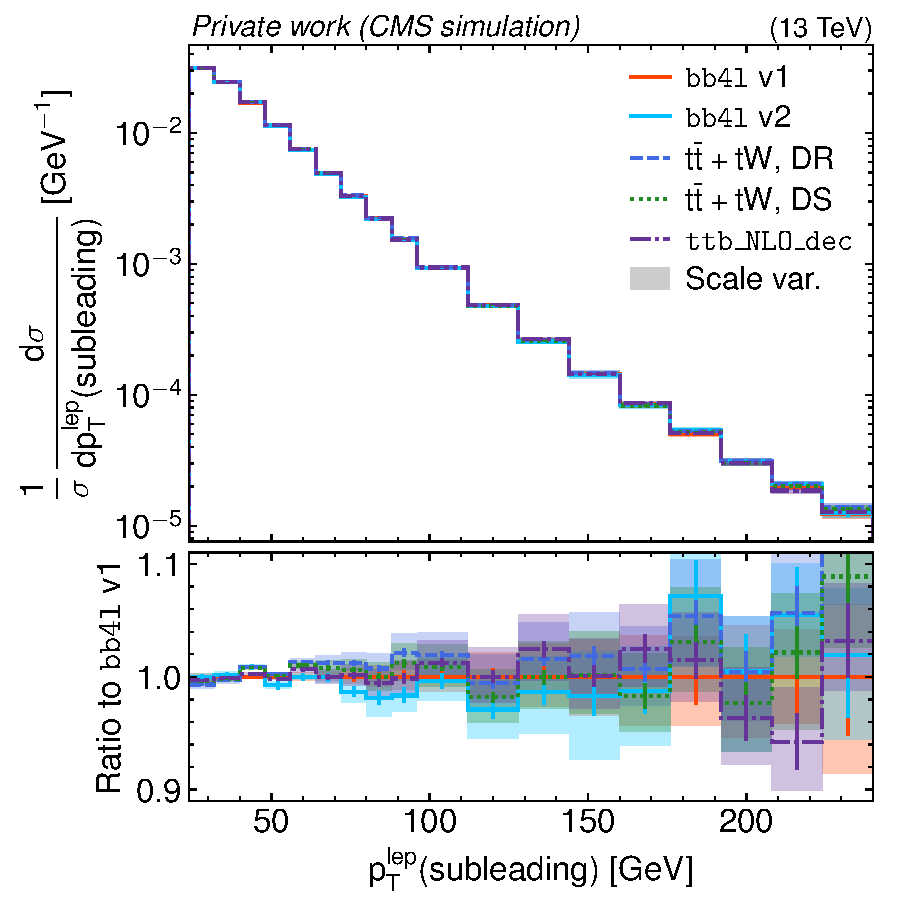
\includegraphics[width=0.49 \textwidth]{figures/bb4l/generators/MC_TTBAR_DILEP_SPINDENSITY_lep_pt_2.pdf}
    \caption{\textbf{Distributions of lepton \pt} of the leading (left) and subleading
      (right) lepton for
      \bbfourl v1 (red), v2 (aqua), \tttWsum with the DR (blue) and DS scheme
      (green), as well as \ttb (magenta). The shaded bands show the
      uncertainty due to scale variations, while the error bars show
      the statistical uncertainty. \textit{Figure adapted from \citere{CMS:NOTE-2023-015}}.}
    \label{fig:bb4l:leppt}
\end{figure}

The same trend can be seen in \cref{fig:bb4l:mll} for the invariant lepton mass \mll, both inclusively and split by lepton flavor channels. The per-channel distributions are all comparable within statistical uncertainties, which validates the extension to same-flavor leptons for \bbfourl presented in \cref{sec:bb4l:sameflavor}.

\begin{figure}[tp]
    \centering
    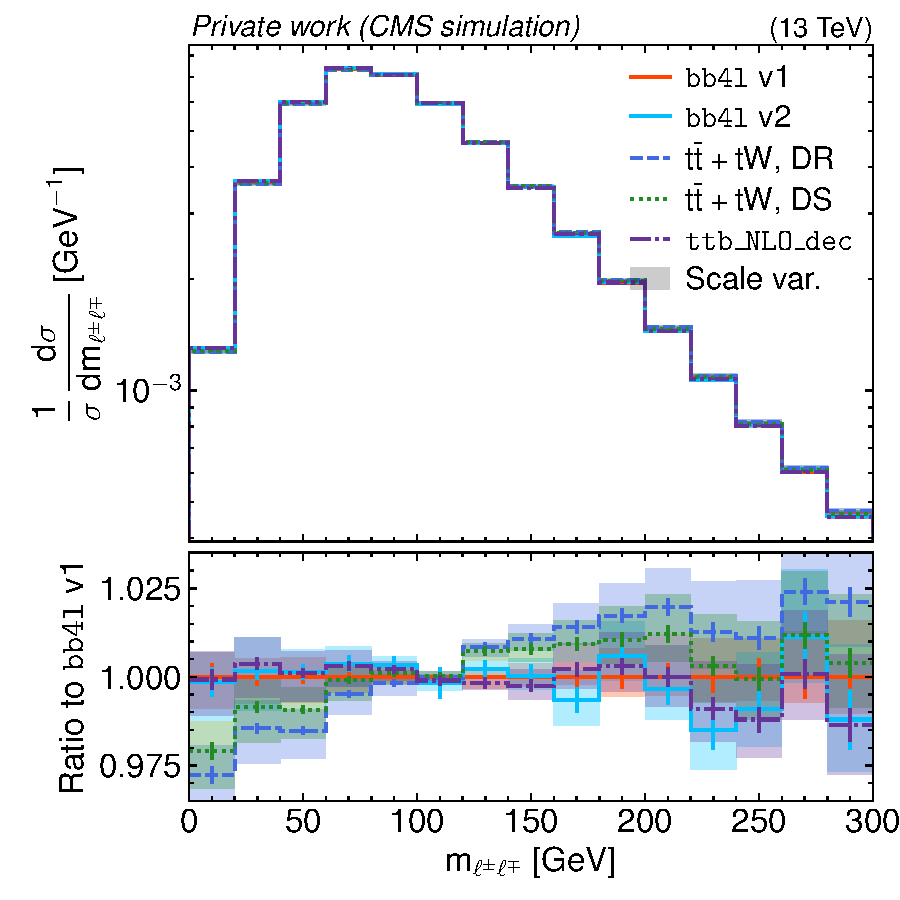
\includegraphics[width=0.49 \textwidth]{figures/bb4l/generators/MC_TTBAR_DILEP_SPINDENSITY_mll.pdf}
    \hfill
    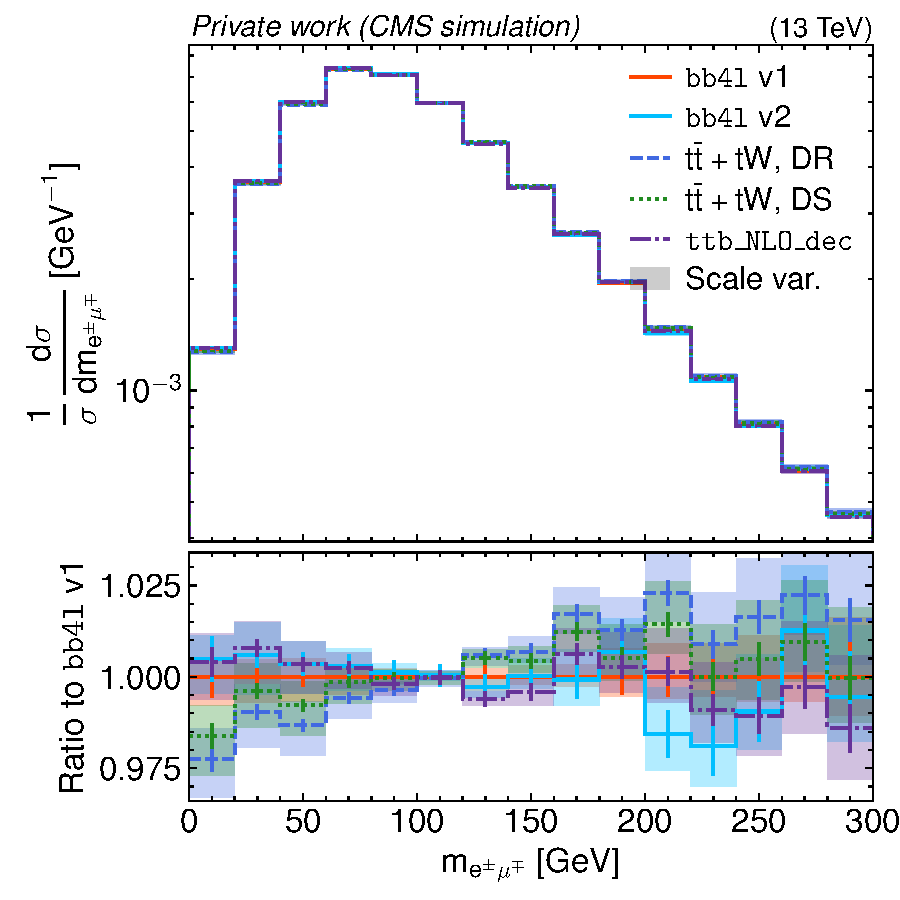
\includegraphics[width=0.49 \textwidth]{figures/bb4l/generators/MC_TTBAR_DILEP_SPINDENSITY_mll_emu.pdf}
    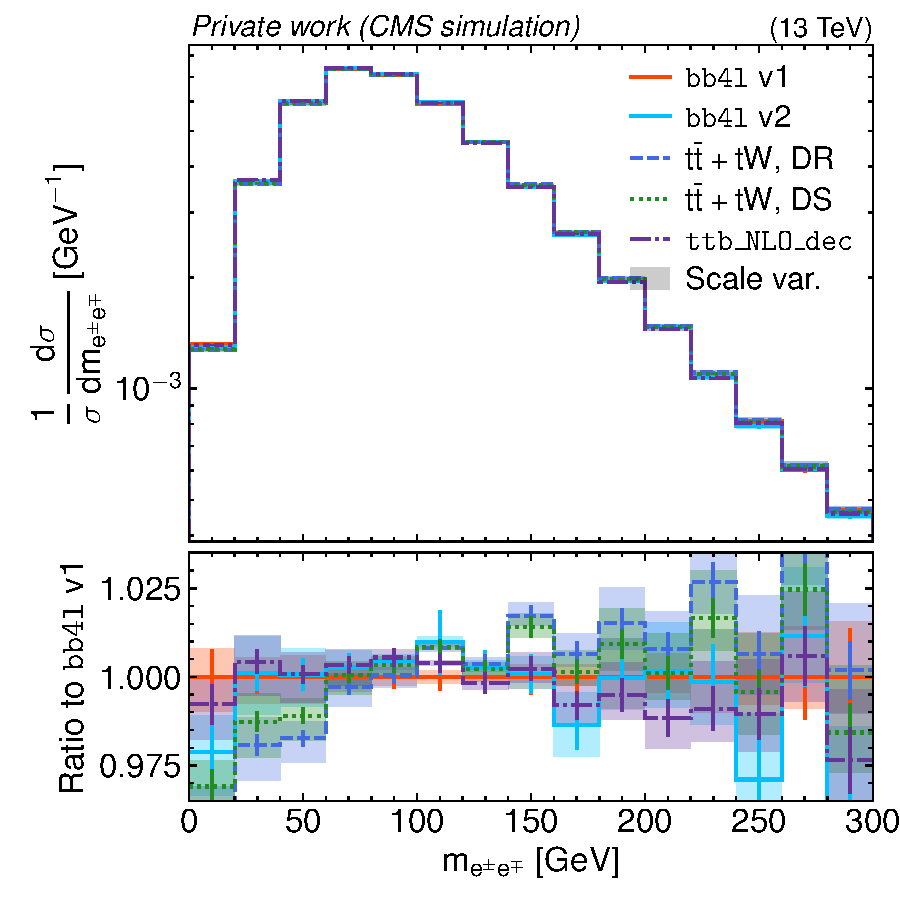
\includegraphics[width=0.49 \textwidth]{figures/bb4l/generators/MC_TTBAR_DILEP_SPINDENSITY_mll_ee.pdf}
    \hfill
    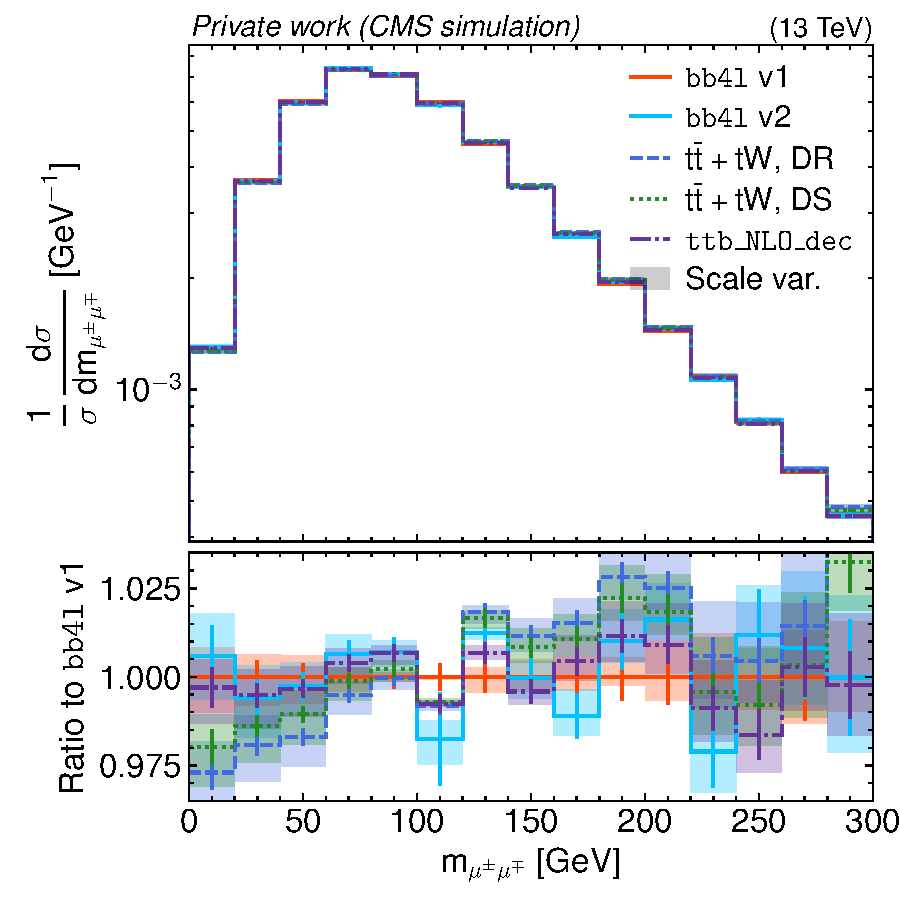
\includegraphics[width=0.49 \textwidth]{figures/bb4l/generators/MC_TTBAR_DILEP_SPINDENSITY_mll_mumu.pdf}
    \caption{\textbf{Distributions of \mll} for all lepton flavors combined (upper left) as well as in the \emu (upper right), \ee (lower left) and \mumu channels (lower right), shown in the same manner as in \cref{fig:bb4l:leppt}. \textit{Figure adapted from \citere{CMS:NOTE-2023-015}}.}
    \label{fig:bb4l:mll}
\end{figure}

\paragraph{Jet observables} Next, some selected AK4 jet observables are compared. 
%For this purpose, the jets are obtained with an anti-$k_\mathrm{T}$ algorithm with distance parameter $\Delta R = 0.4$ (AK4)~\cite{Cacciari:2008gp}.
Jets containing a B hadron are identified as b jets using a ghost association technique~\cite{Cacciari:2007fd,Cacciari:2008gn}. 

\begin{figure}[tp]
    \centering
    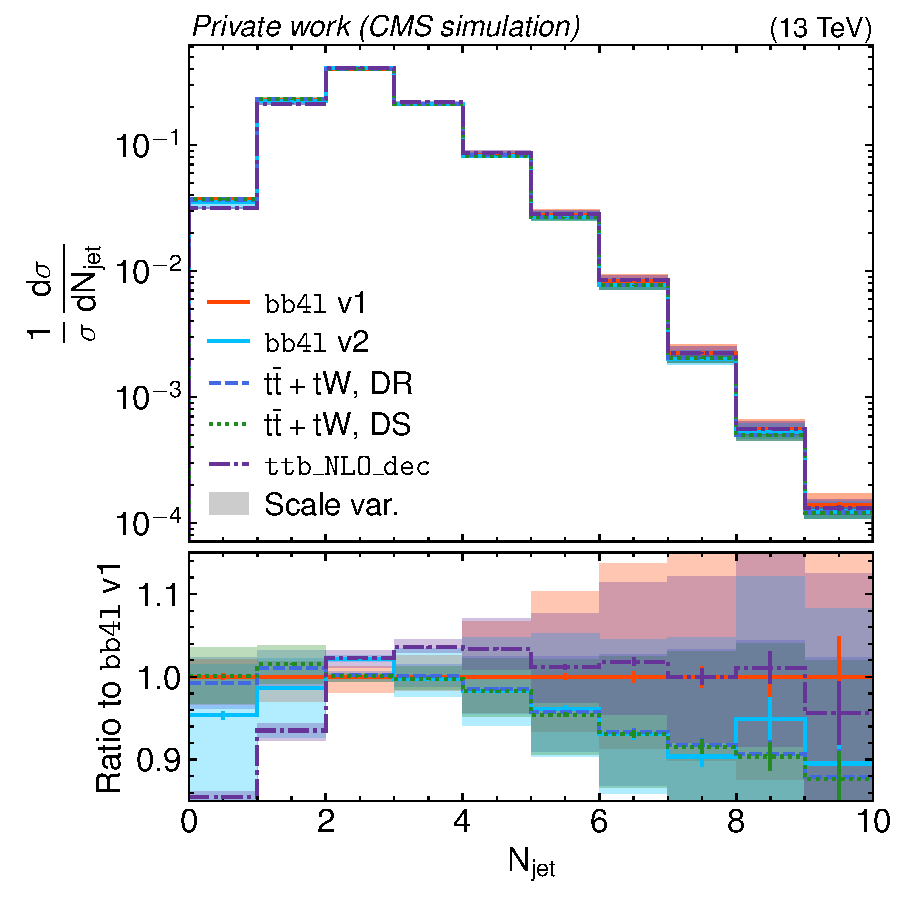
\includegraphics[width=0.49 \textwidth]{figures/bb4l/generators/MC_TTBAR_DILEP_SPINDENSITY_njet.pdf}
    \hfill
    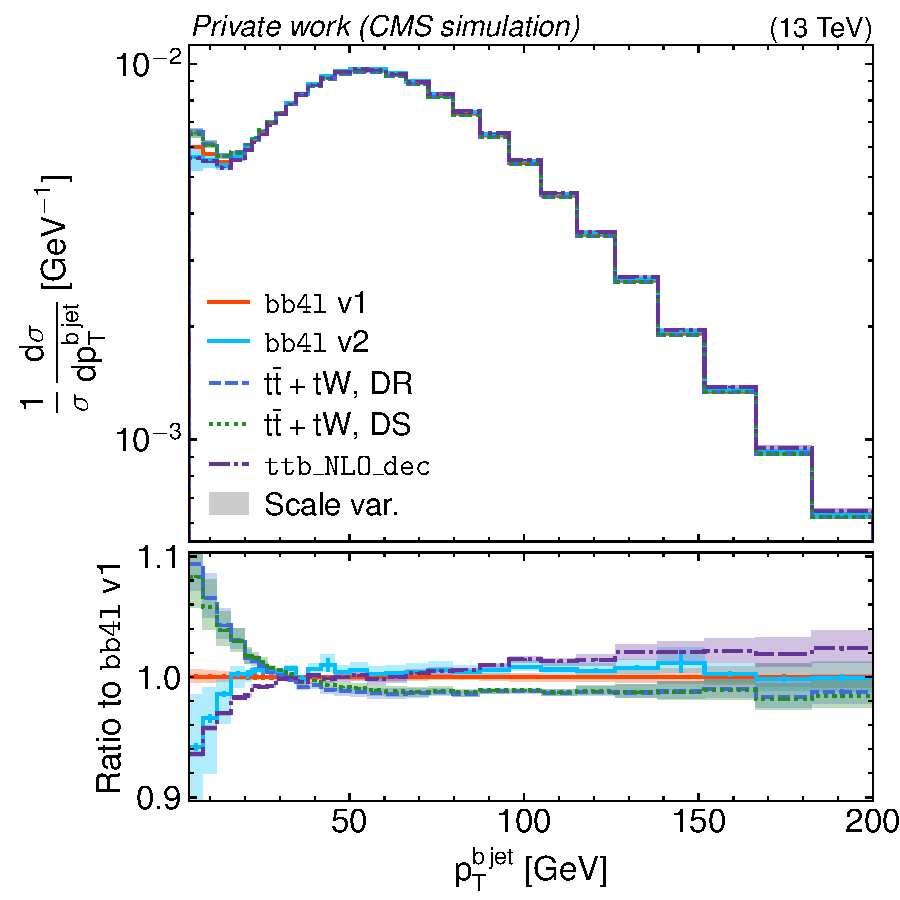
\includegraphics[width=0.49 \textwidth]{figures/bb4l/generators/MC_HFJETS_ptBJetLead.pdf}
    \caption{\textbf{Number of jets and b jet \pt}. Distributions of the inclusive number of AK4 jets (left) and the \pt of the leading b jet (right, \rivet analysis \texttt{MC\_HFJETS}), shown in the same manner as in \cref{fig:bb4l:leppt}. \textit{Figure adapted from \citere{CMS:NOTE-2023-015}}.}
    \label{fig:bb4l:jets1}
\end{figure}

\begin{figure}[tp]
    \centering
    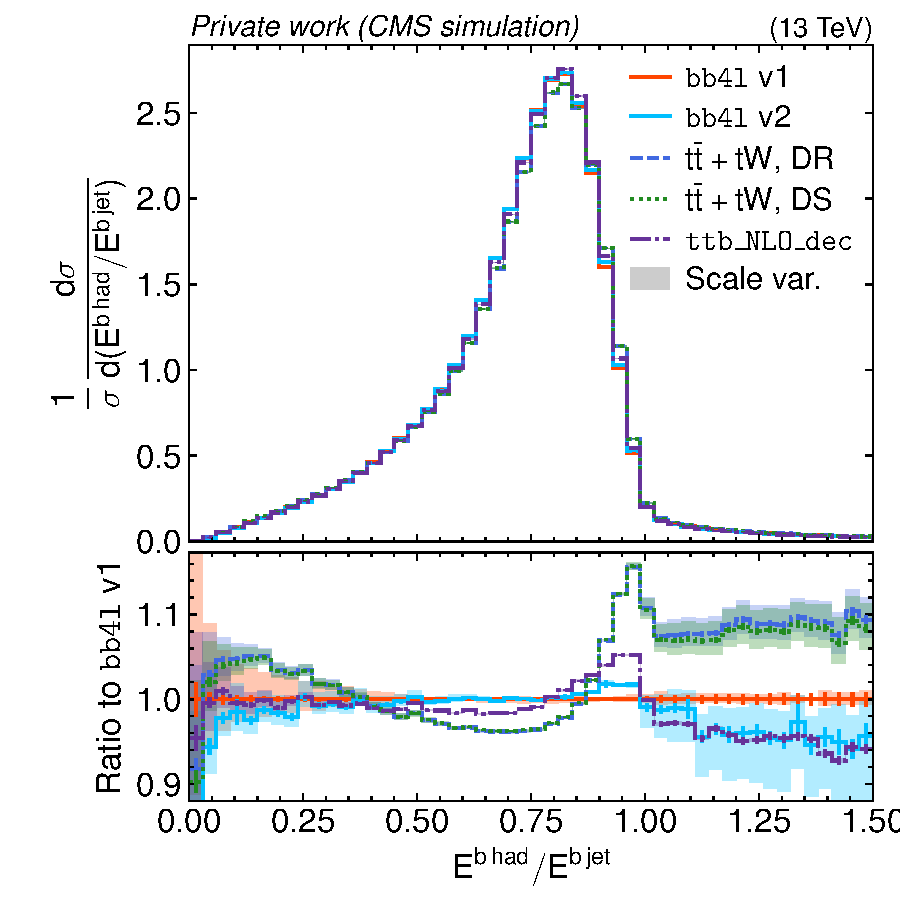
\includegraphics[width=0.49 \textwidth]{figures/bb4l/generators/MC_HFJETS_efracB.pdf}
    \hfill
    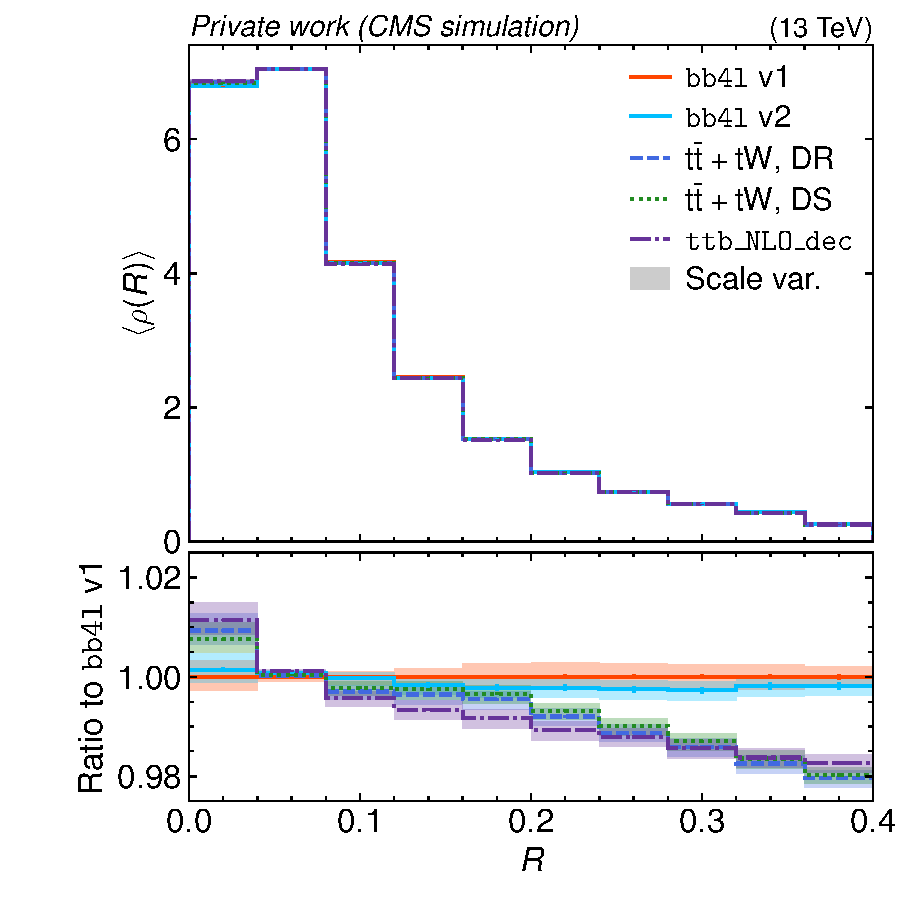
\includegraphics[width=0.49 \textwidth]{figures/bb4l/generators/MC_HFDECAYS_avg_rho_B_jet.pdf}
    \caption{\textbf{b fragmentation and jet shape.} Distributions of the b quark fragmentation (left, \rivet analysis \texttt{MC\_HFJETS}) and the average differential b jet shape (right, \rivet analysis \texttt{MC\_HFDECAYS}), shown in the same manner as in \cref{fig:bb4l:leppt}. \textit{Figure adapted from \citere{CMS:NOTE-2023-015}}.}
    \label{fig:bb4l:jets2}
\end{figure}

\cref{fig:bb4l:jets1} shows the inclusive number of jets and the \pt of the leading b jet for the different cases. Several differences are observable here both between the two versions of \bbfourl and between \bbfourl and the other generators. For the number of jets, these are mostly covered by the scale uncertainties, while for the b jet \pt, there is an uncovered discrepancy at very low \pt. It is interesting to note that the number of jets agrees well between \tttWsum and \bbfourl v2, while \bbfourl v1 and \ttb disagree and predict a larger number of jets. The origin of these discrepancies, especially between the \bbfourl versions, is not yet understood.

Next, \cref{fig:bb4l:jets2} shows the b quark fragmentation, defined as the fraction of energy of the central B hadron in a jet compared to the total jet energy, as well as the average differential b jet shape $\langle \rho (R) \rangle$, which is the density of particles making up the b jet as a function of its radius $R$. Both of these variables are sensitive to final-state radiation from the top decay, and are thus expected to be affected by the full NLO calculation performed by \bbfourl. It can be seen that both versions of \bbfourl predict softer b jet spectra and wider jets than both \tttWsum and \ttb, which can be interpreted as more FSR emissions being generated. Notably, this effect cannot be solely due to the inclusion of hard FSR emissions in \bbfourl since these are also present in \ttb.

In general, all of these trends for \bbfourl (softer lepton and b jet spectra as well as wider jets) agree with what was observed in Refs.~\cite{FerrarioRavasio:2018whr,ATLAS:PHYS-PUB-2021-042}, but differ from the results initially reported in \citere{Jezo:2016ujg}.

\paragraph{Invariant b$\ell$ mass} A common proxy observable to use for measurements of the top quark mass in dilepton events is the invariant mass \mbl of a b jet and a lepton. To do so, a procedure is needed to unambiguously assign the leptons and b jets (of which there might be varying numbers per event depending on the event selection) to each other. Here, exactly two b jets per event are required, and the so-called minimax mass is used, defined as

\begin{equation}
    \mblminimax = \min{ \left[  \max{ \left( m_{b_1 \ell_1},
          m_{b_2 \ell_2} \right) }, \max{ \left( m_{b_1 \ell_2},
          m_{b_2 \ell_1} \right) } \right] }.
\end{equation}

This prescription amounts to maximizing over the two b-$\ell$ pairs in the event, and then minimizing over the two possible assignments of b jets and leptons. It is notable in that, for double-resonant \ttbar events, it shows a kinematic cutoff at a value of $\sqrt{\smash[b]{m_t^2 - m_W^2}} \approx \SI{150}{\GeV}$. As a result, the tail above this cutoff is sensitive to single-resonant tW events as well as \tttW interference and thus to the top quark width.

\begin{figure}[tp]
    \centering
    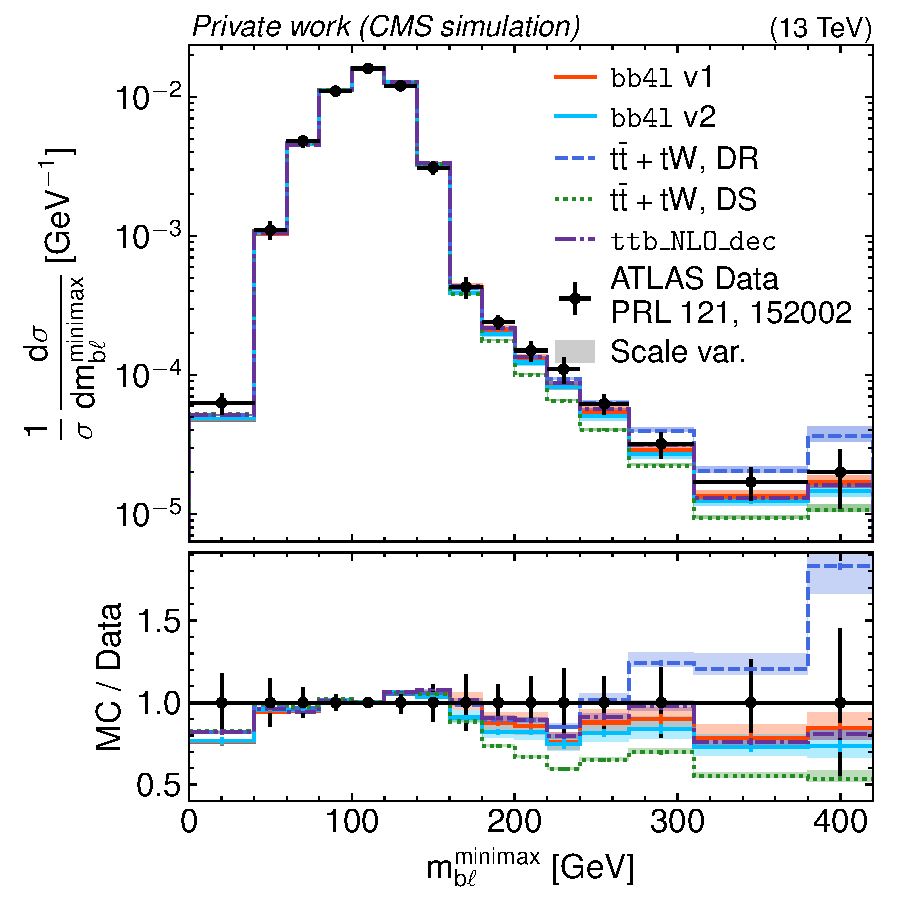
\includegraphics[width=0.49 \textwidth]{figures/bb4l/generators/ATLAS_2018_I1677498_d03-x01-y01.pdf}
    \caption{\textbf{Distribution of \mblminimax}, shown in the same manner as in \cref{fig:bb4l:leppt}. ATLAS data from \citere{ATLAS:2018ivx} is overlaid as black dots, and the \rivet routine from said reference was used to obtain the distributions. \textit{Figure adapted from \citere{CMS:NOTE-2023-015}}.}
    \label{fig:bb4l:mbl}
\end{figure}

\cref{fig:bb4l:mbl} shows the distribution of \mblminimax, again for all considered cases. It can be seen that both versions of \bbfourl in good agreement with each other, and are also in agreement with \ttb except for the lowest bin. Unfolded ATLAS data taken from \citere{ATLAS:2018ivx} is overlaid on top of the predictions, and shows good agreement for both \bbfourl and \ttb. 
In the tail, the two interference handling schemes for \tttWsum show significant differences as expected, with \bbfourl and \ttb lying between them. Since \bbfourl is expected to provide a more accurate prediction of the interference then either scheme, this validates that using the difference of the schemes as an uncertainty covers the true values, as is done in many CMS and ATLAS measurements. Going forward, such uncertainties could be dropped from future measurements by using \bbfourl predictions directly.

\paragraph{Top quark reconstruction} Finally, in order to directly study the effects on top quark observables, a simple generator-level top quark reconstruction is performed. To do so, two dressed leptons and two b jets are selected as before, while the two neutrinos in the dileptonic top decay are taken from truth-level information. The W bosons are reconstructed from the neutrinos and charged leptons according to the lepton charge, and then combined with the b jets to form two possible assignments of b-W pairs, which are taken as top quark and antiquark candidates again depending on the lepton charge. The ambiguity in assignments is resolved by choosing the pairs for which the difference $\Delta m_t$ between the invariant masses is minimized. 

This reconstruction procedure is not equivalent to a full experimental reconstruction, in which the neutrinos are only measured as missing transverse momentum and can thus not be directly assigned to the leptons. It also does not include any detector resolution effects. However, it does take into account the effects of FSR in the top decay by considering the full b jets instead of parton-level b quarks, which is why it was chosen for the comparison.

\begin{figure}[tp]
    \centering
    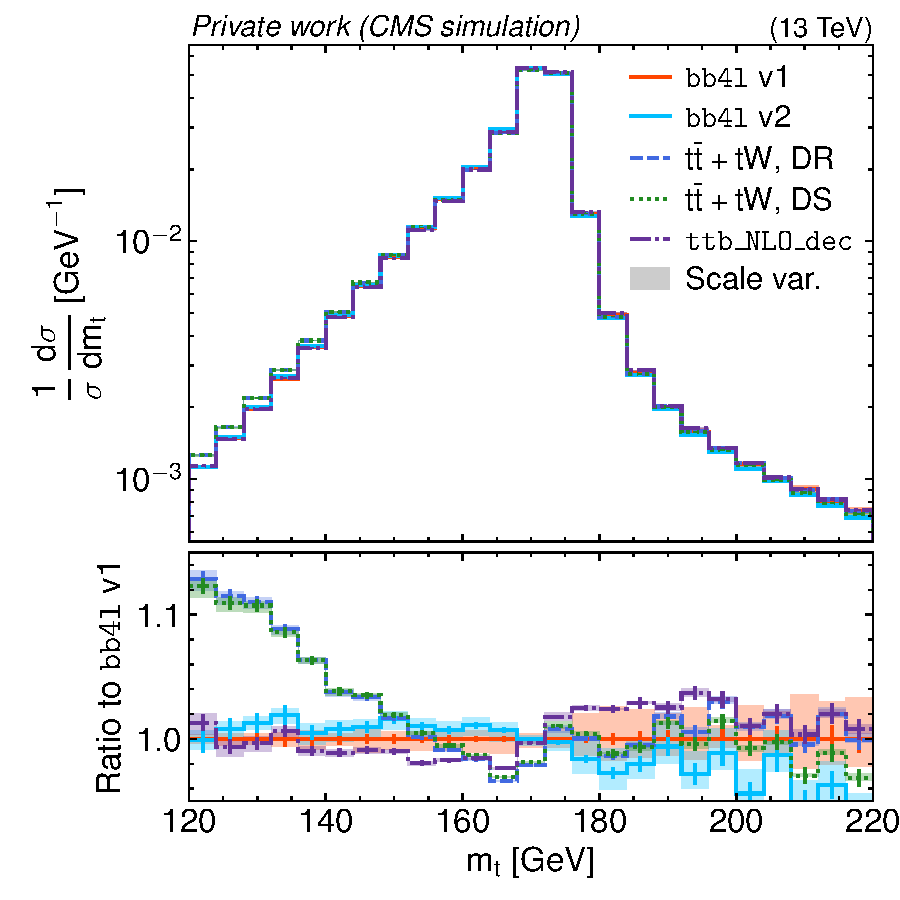
\includegraphics[width=0.49 \textwidth]{figures/bb4l/generators/MC_TTBAR_DILEP_SPINDENSITY_anytop_mass.pdf}
    \hfill
    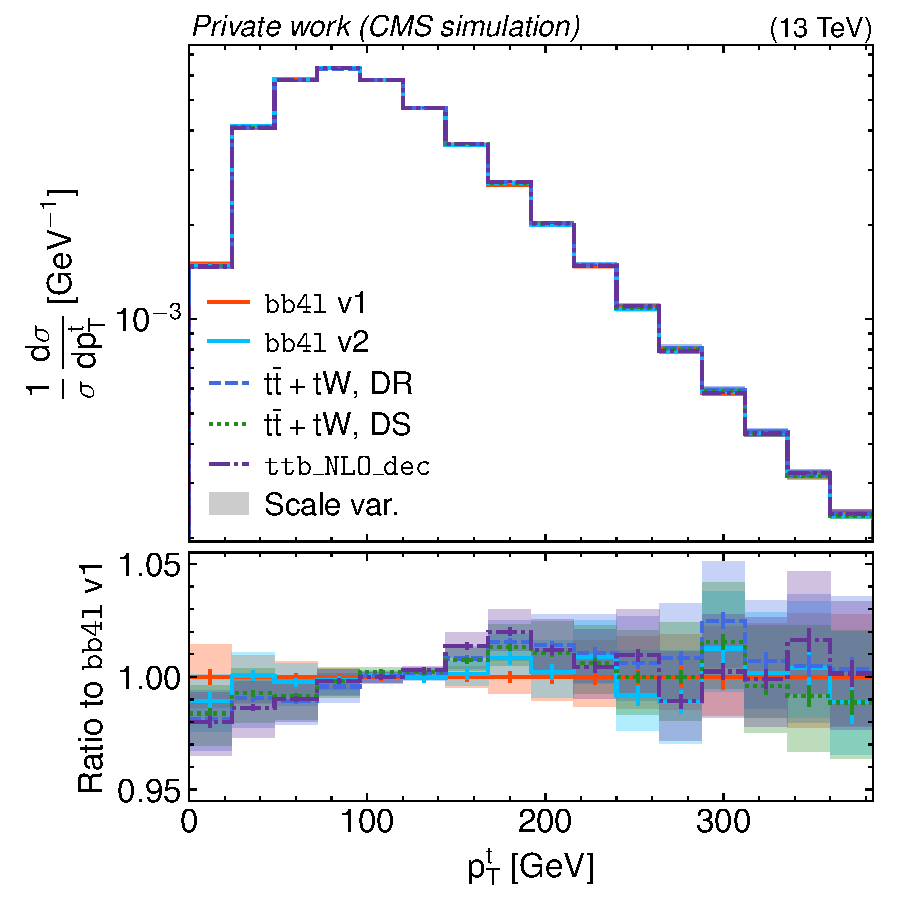
\includegraphics[width=0.49 \textwidth]{figures/bb4l/generators/MC_TTBAR_DILEP_SPINDENSITY_anytop_pt.pdf}
    \caption{\textbf{Top quark lineshape and \pt.} Distributions of the reconstructed top quark mass (left) and \pt (right), summed for both top quark and antiquark, shown in the same manner as in \cref{fig:bb4l:leppt}. \textit{Figure adapted from \citere{CMS:NOTE-2023-015}}.}
    \label{fig:bb4l:top}
\end{figure}

\cref{fig:bb4l:top} shows the resulting distributions for the top quark mass and \pt. It can be seen that the different generators show different lineshapes for the top quark mass: \bbfourl predicts a small shift towards lower values compared to \tttWsum for both interference handling schemes as well as \ttb, and also predicts significantly lower amounts of off-shell tops with masses below the pole mass compared to \tttWsum. Both of these facts are important for precision top mass measurements, in which such shifts can influence the final fit results. The presense of these differences is expected: due to the use of the NWA for both \tttWsum and \ttb, the top lineshape can only be modeled approximately in these generators, while \bbfourl provides a true NLO-accurate description. It can furthermore be seen that the two \bbfourl versions are not in perfect agreement with each other, though the difference is within the scale uncertainties by 1 standard deviation.

For the top quark \pt, on the other hand, any trend in the comparison between the generators is covered by the scale uncertainties, though \bbfourl does seem to again predict softer \pt spectra than the other generators, consistent with the trends observed for the lepton \pt and \mll.

\begin{figure}[tp]
    \centering
    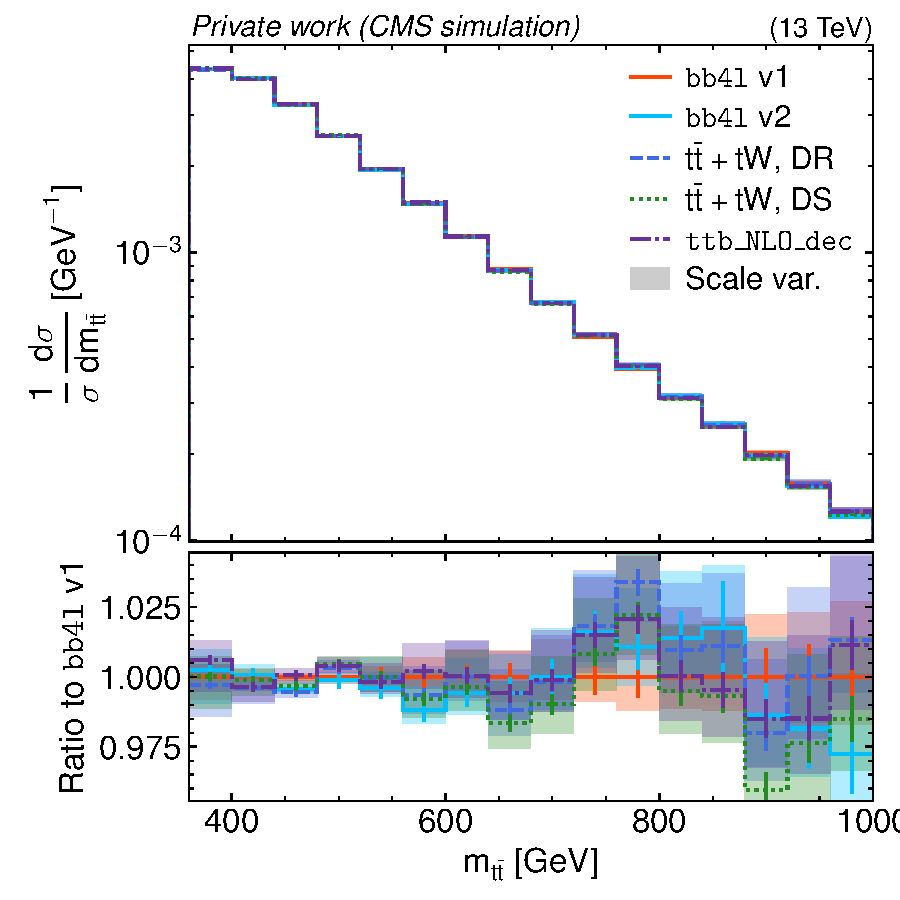
\includegraphics[width=0.49 \textwidth]{figures/bb4l/generators/MC_TTBAR_DILEP_SPINDENSITY_ttbar_mass.pdf}
    \hfill
    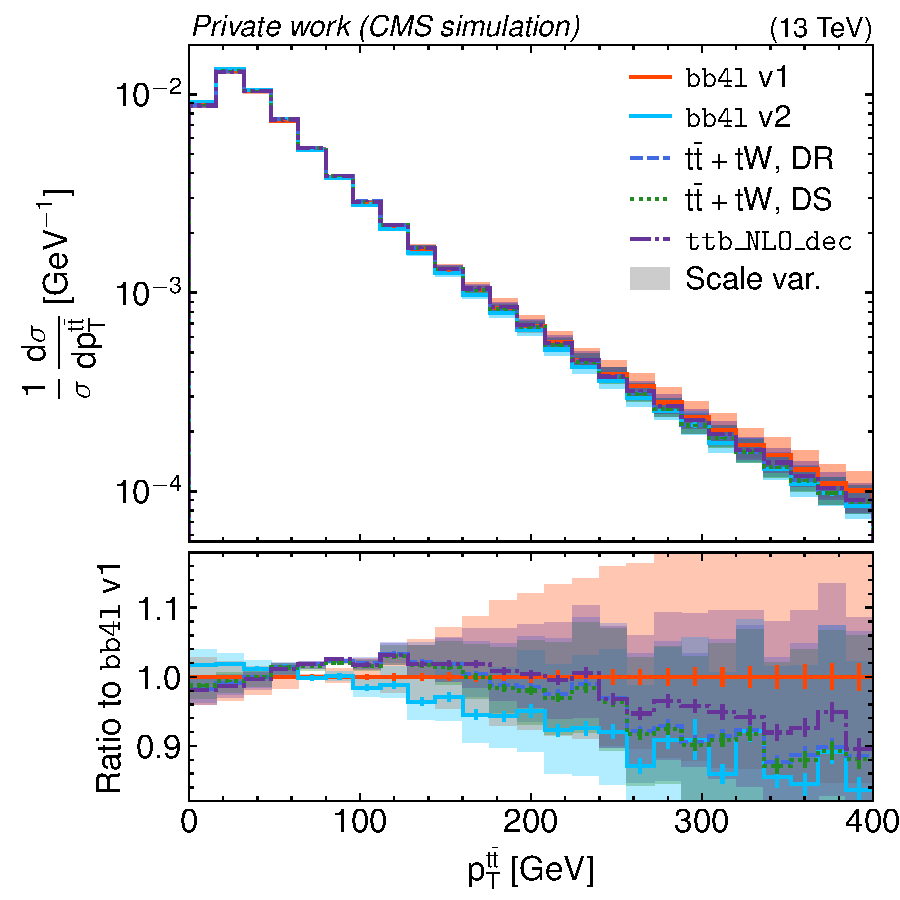
\includegraphics[width=0.49 \textwidth]{figures/bb4l/generators/MC_TTBAR_DILEP_SPINDENSITY_ttbar_pt.pdf}
    \caption{\textbf{Kinematics of the \ttbar system.} Distributions of the reconstructed invariant mass (left) and \pt (right) of the \ttbar system, shown in the same manner as in \cref{fig:bb4l:leppt}. \textit{Figure adapted from \citere{CMS:NOTE-2023-015}}.}
    \label{fig:bb4l:ttbar}
\end{figure}

Lastly, the invariant mass and \pt distributions of the \ttbar system as a whole are shown in \cref{fig:bb4l:ttbar}. For \mtt, no clear trend can be seen for any of the considered generators. The \pt of the \ttbar system, on the other hand, shows significant differences both between the two \bbfourl versions and between \bbfourl and the other generators (which agree with each other). It should be noted that, since the initial state of the \pptt process has negligible \pt, this variable is exactly zero at LO in QCD, and consequently determined only by emissions at NLO and beyond. As a result, it is expected to be sensitive to the NLO calculation and matching between matrix element and parton shower.

\subsection{Comparison of FSR matching settings}
\label{sec:bb4l:matching}

Complementary to the previous generator comparisons, this section investigates the effect of the matching between matrix element and parton shower for FSR in \bbfourl. As explained in \cref{sec:bb4l:matching_theory}, two principal options are available to match \bbfourl to \pythia in the used module \texttt{PowhegHooksBB4L}: In the first and nominal approach (denoted ``FSR veto''), the parton shower is started at the kinematic limit, and FSR emissions that lie above the \powheg energy scale of the relevant emission from the top decay as generated by \powheg are vetoed. In the second approach (``Res. scale''), the shower is directly started at the energy scale of the \powheg FSR emission, neglecting the mismatch between scale definitions in \powheg and \pythia. 

In order to demonstrate the importance of correct parton shower matching, a third case (``Kin. limit'') is considered, in which the parton shower for FSR emissions is started naively at the kinematic limit without any veto procedure specifically directed at \bbfourl. This approach is thus expected to double-count FSR emissions.

The comparison in this section has been performed with \bbfourl v1. The matching for ISR emissions, done by \texttt{PowhegHooks}, is left identical between the three cases, as given in \cref{tab:bb4l:settings}.

\begin{figure}[tp]
    \centering
    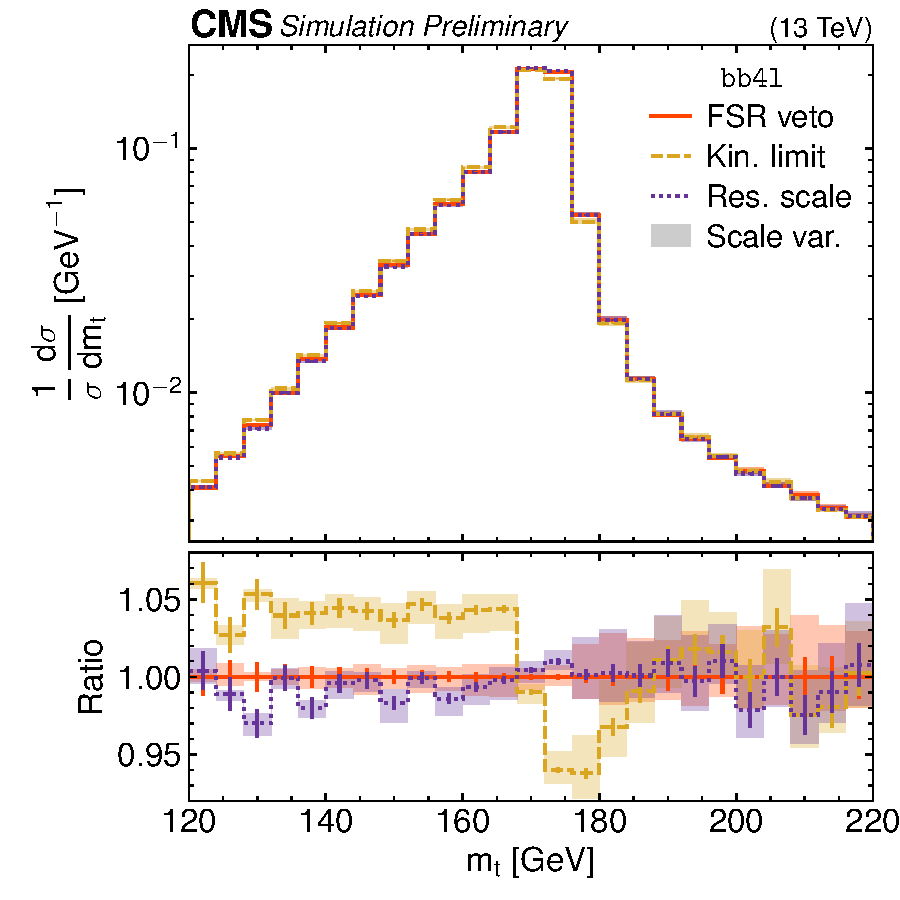
\includegraphics[width=0.49 \textwidth]{figures/bb4l/matching/ADDED_top_mass.pdf}
    \hfill
    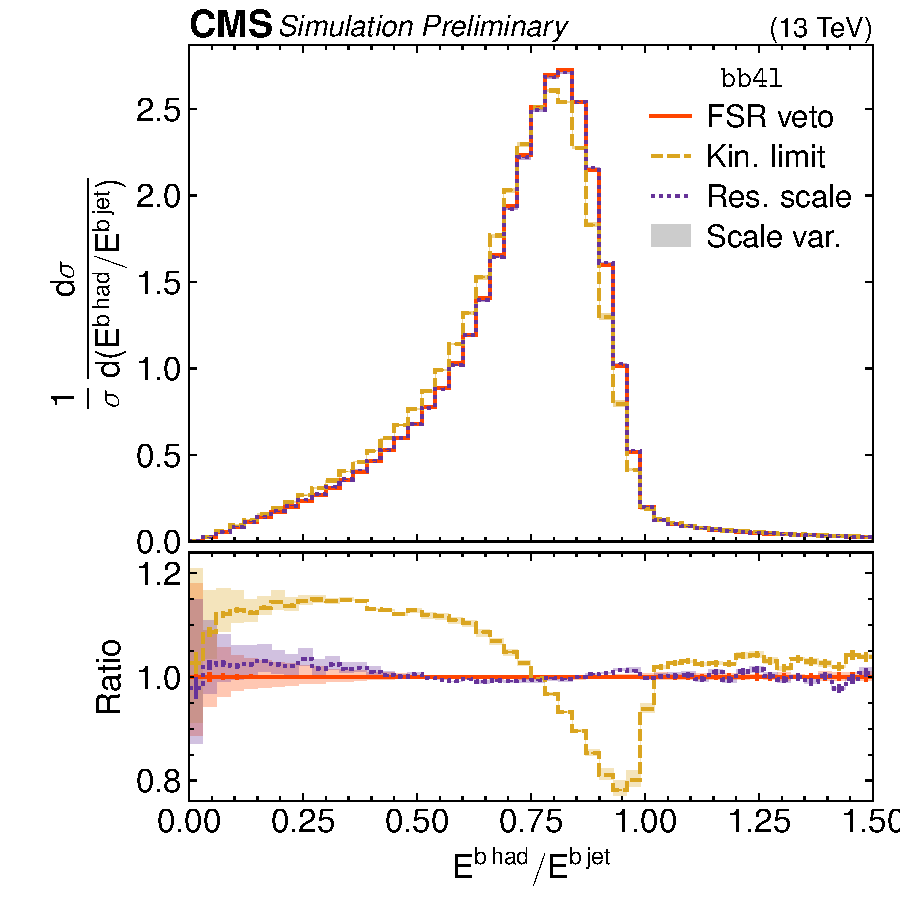
\includegraphics[width=0.49 \textwidth]{figures/bb4l/matching/MC_HFJETS_efracB.pdf}
    \caption{\textbf{Comparison of FSR matching settings.} Distributions of the reconstructed top quark mass (left, same as in \cref{fig:bb4l:top}) and the b quark fragmentation (right, same as in \cref{fig:bb4l:jets2}), for \bbfourl with different FSR matching settings as explained in the text (\cref{sec:bb4l:matching}). The shaded bands show scale uncertainties. \textit{Figure taken from \citere{CMS:NOTE-2023-015}}.}
    \label{fig:bb4l:matching}
\end{figure}

\cref{fig:bb4l:matching} shows the distributions of the top quark mass, reconstructed the same as before, and the b fragmentation for the different matching choices. Both of these observables were chosen for their sensitivity to FSR effects. It can be seen that the options ``FSR veto'' and ``Res. scale'' agree reasonably well with each other, with the top mass lineshape showing a small shift between them within the scale uncertainties. This implies that the mismatch between the \powheg and \pythia energy scale definitions has a subleading effect in practice. On the other hand, the naive ``Kin. limit'' approach shows a large discrepancy due to its double-counting of FSR emissions, highlighting the importance of correct matching FSR matching procedures for NLO generators.

\subsection{Recoil in top decay}
\label{sec:bb4l:recoil}

In the simple parton shower in \pythia, there is a well-known problem affecting the virtualities of heavy unstable colored resonances, such as the top quark, in the treatment of FSR emissions in the resonance decay~\cite{Brooks:2019xso}. In particular, when performing a gluon emission off the decaying top quark and thus changing a $t \rightarrow Wb$ configuration to $t \rightarrow Wbg$, there is an ambiguity on how to distribute the recoil imposed by the gluon between the top decay products (W and b quark) such that the four-momentum of the $Wbg$ system is conserved.

\pythia 8.307, which is the version used for the previous studies in this chapter, offers two different treatments for this problem, which amount to assigning the recoil to only the W (``recoil to W'') or only to the b quark (``recoil to b''). Both of these are approximations, since a true treatment would distribute the recoil between the W and b quark in some form. CMS, and thus the studies previously shown in this chapter, use the ``recoil to b'' option.

Since \pythia 8.310, a third option (``recoil to top'') has been made available via the setting \texttt{TimeShower:recoilStrategyRF}. For this option, the W is chosen as the recoiler at first, but the emissions are then reweighted according to the ratios of eikonal radiation factors to approximate the radiation pattern expected in a resonance-aware shower~\cite{Brooks:2019xso}. It has been found in \citere{ATLAS:2022jbw} that the difference between this improved method and the old ones can have a substantial impact on top mass proxy observables and consequently measured top mass values, and it has been discussed whether such a difference should be included as a systematic uncertainty.

This problem, in its core, is an issue of the parton shower and not the ME generator. Nonetheless, \bbfourl is expected to alleviate some of the ambiguities since it always includes the hardest gluon emission in each top decay at the ME level, where no question of assigning the recoil is raised. For subsequent and thus subleading emissions, the issue in principle still persists.

To estimate the effect of the top recoil in \bbfourl and compare it to \tttWsum, events from both generators are re-showered in \pythia 8.310 with the two choices of setting
\begin{align*}
\begin{split}
  \texttt{TimeShower:recoilStrategyRF = 1} &\quad \text{(``recoil to b'')} \quad \text{and} \\
  \texttt{TimeShower:recoilStrategyRF = 2} &\quad \text{(``recoil to top'')}.
\end{split}
\end{align*}
\bbfourl v2 is used for this comparison, and all other settings are kept at the nominal. For \tttWsum, only the DR scheme is considered for the interference handling.

\begin{figure}[tp]
    \centering
    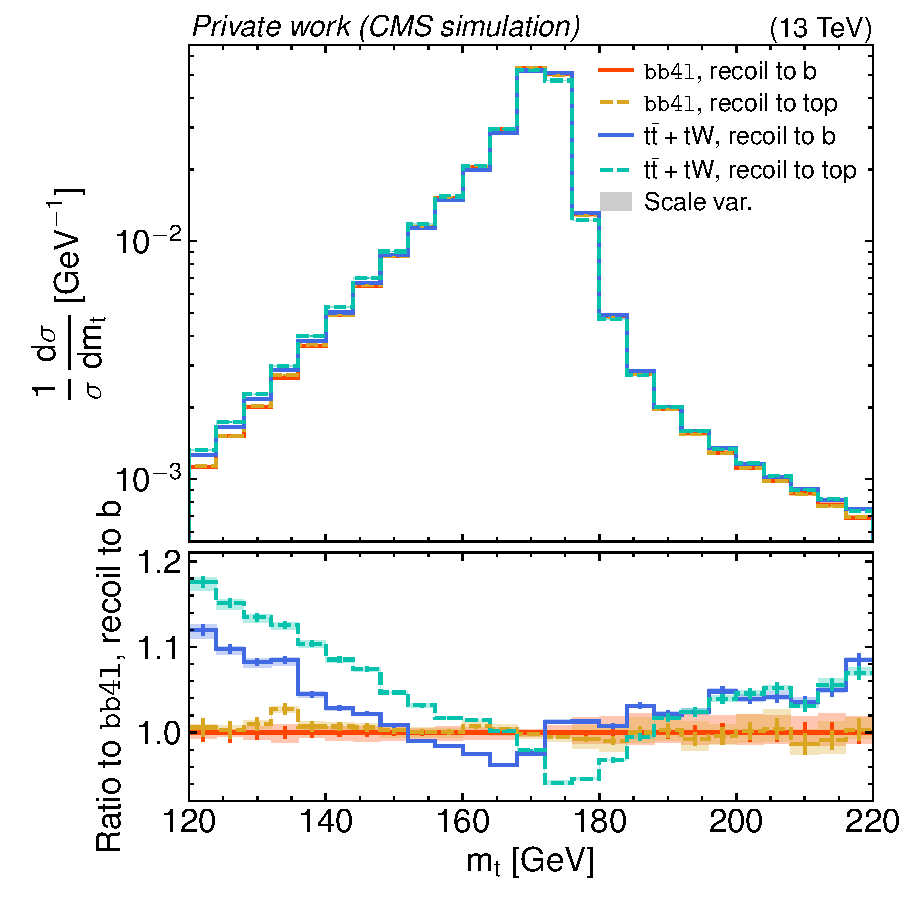
\includegraphics[width=0.49 \textwidth]{figures/bb4l/recoil/MC_TTBAR_DILEP_SPINDENSITY_anytop_mass.pdf}
    \hfill
    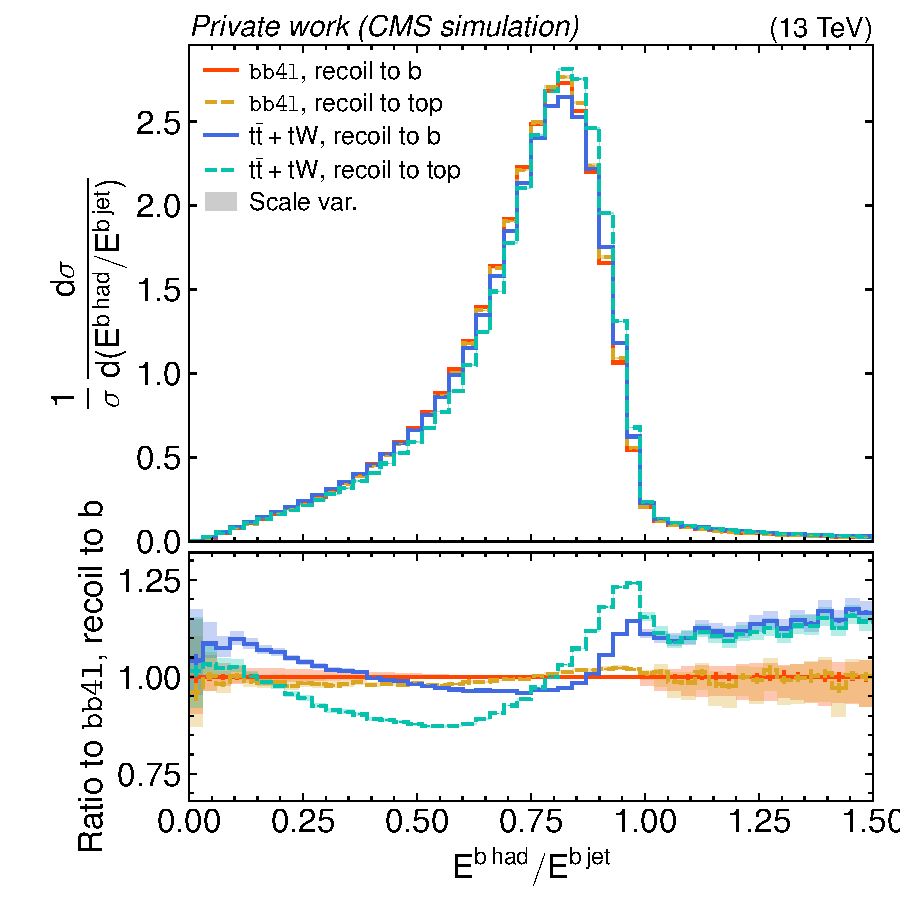
\includegraphics[width=0.49 \textwidth]{figures/bb4l/recoil/MC_HFJETS_efracB.pdf}
    \caption{\textbf{Comparison of top recoil strategies.} Distributions of the reconstructed top quark mass (left, same as in \cref{fig:bb4l:top}) and the b quark fragmentation (right, same as in \cref{fig:bb4l:jets2}), for \bbfourl and \tttWsum with two different recoil treatments, as defined in the text (\cref{sec:bb4l:recoil}). The shaded bands show scale uncertainties.}
    \label{fig:bb4l:recoil}
\end{figure}

The results are shown in \cref{fig:bb4l:recoil} for the reconstructed top mass and the b quark fragmentation. Large differences are visible between the two recoil strategies for \tttWsum, as expected from Refs.~\cite{Brooks:2019xso,ATLAS:2022jbw}. For \bbfourl, on the other hand, the differences are almost invisible, and lie within the scale uncertainties for the top quark mass. This implies that the effect of the recoil in subleading emissions is negligible in \bbfourl for the shown observables. As a result, \bbfourl fully circumvents the problem of top recoil that can otherwise be significant for \ttbar analyses.

\section{Summary and Outlook}

In this chapter, several generator-level studies of the MC generator \bbfourl, which generates the full $b \bar{b} \ell^+ \ell^- \nu_{\ell} \bar{\nu}_{\ell}$ final state including \tttW interference and off-shell top effects at NLO in QCD, have been presented. \bbfourl has been compared to other common \ttbar generators, namely \hvq, \ST (with two interference handling schemes) and \ttb, for different lepton, (b) jet and reconstructed top quark observables. For \mblminimax, \bbfourl agrees well with ATLAS data from \citere{ATLAS:2018ivx}, improving greatly upon the two interference handling schemes DR and DS for \tttWsum. For the reconstructed top quark mass, \bbfourl shows a significant shift compared to \tttWsum. In addition, two different \bbfourl versions have been compared, with no significant differences found outside of scale uncertainties, and the matching of ME and parton shower as well as the treatment of the recoil in \bbfourl have been studied further.

These studies represent valuable information for the choice of \ttbar MC generator in upcoming CMS measurements. For analyses in which \ttbar and tW are major backgrounds, \bbfourl can help reduce uncertainties originating in the \tttW interference treatment, and provide a more accurate description when off-shell regions of phase space are probed. This is briefly explored in \cref{sec:ah:gennps} in the context of a search for \ttbar bound state effects, which are naturally located in an off-shell-region. Furthermore, \bbfourl will be of use when the \pptt process is instead the signal of a measurement. In particular, for future work it would be interesting to perform a simultaneous top mass and width measurement using MC templates generated with \bbfourl, as originally proposed in \citere{FerrarioRavasio:2018whr}, in CMS, or alternatively perform an differential \tttWsum cross section measurement, where \bbfourl could be used to unfold the data to generator level. 
%However, both of these ideas are outside the scope of this thesis, and are left for future work.